\documentclass{llncs}

% -----------------------------------------------------------------------------
% Geometry and Margins (Guideline 10: A4 paper, top/bottom 2.05 in, left/right 1.73 in)
% -----------------------------------------------------------------------------
\usepackage[a4paper,top=2.05in,bottom=2.05in,left=1.73in,right=1.73in]{geometry}

% -----------------------------------------------------------------------------
% Font and Encoding (Times font family as prescribed in LNCS template)
% -----------------------------------------------------------------------------
\usepackage[utf8]{inputenc}
\usepackage[T1]{fontenc}
\usepackage{mathptmx}

% -----------------------------------------------------------------------------
% Essential Packages
% -----------------------------------------------------------------------------
\usepackage{graphicx}
\usepackage{amsmath,amssymb,amsfonts}
\usepackage{booktabs}
\usepackage{array}
\usepackage{url}
\usepackage{cite}
\usepackage{microtype}

\graphicspath{{figures/}{./}}

% -----------------------------------------------------------------------------
% Guideline 6: No page numbering and no running head title
% -----------------------------------------------------------------------------
\pagestyle{empty}

\begin{document}

\pagenumbering{gobble}

% -----------------------------------------------------------------------------
% Title (Guideline 10: 14pt - bold)
% -----------------------------------------------------------------------------
\title{YOLOv8s Enhanced with CBAM Attention and WIoUv2 Loss for Automated Printed Circuit Board Defect Detection}

% -----------------------------------------------------------------------------
% Authors & Affiliations (Guidelines 4 & 5: No social/academic titles, no positions,
% full address, affiliation, email of all authors, corresponding author specified)
% -----------------------------------------------------------------------------
\author{Varsha Sambhaje\inst{1}\thanks{Corresponding author: \email{varsha.s@srmap.edu.in}} \and
Madhira Venkata Ramesh Reddy\inst{1}}

\institute{Department of Computer Science and Engineering, SRM University-AP, \\
Amaravati, Andhra Pradesh 522240, India \\
\email{varsha.s@srmap.edu.in}, \email{ramesh\_madhira@srmap.edu.in}}

\maketitle

% -----------------------------------------------------------------------------
% Abstract (Guideline 7: Single independent paragraph, NO citations, NO section number)
% -----------------------------------------------------------------------------
\begin{abstract}
Automated surface inspection of printed circuit boards (PCBs) is an indispensable quality assurance operation in modern electronics manufacturing, where undetected manufacturing flaws precipitate multi-billion-dollar annual rework liabilities. Conventional automated optical inspection (AOI) relying on template differencing suffers from severe false alarms under illumination drift and board misalignments. While deep convolutional detectors provide real-time throughput, standard architectures suffer from recall degradation on tiny, non-convex defect morphologies due to copper texture clutter and gradient misallocation in conventional bounding-box regression losses. In this investigation, we engineer an enhanced defect localization framework founded upon YOLOv8s, reinforced through two synergistic architectural interventions: (i) dual-branch Convolutional Block Attention Module (CBAM) blocks in the PANet neck for joint spatial and channel saliency calibration; and (ii) Wise-IoU version 2 (WIoUv2) dynamic focusing loss utilizing an Exponential Moving Average (EMA) baseline to allocate optimization budget to challenging instances. Evaluated on the DeepPCB benchmark, the proposed architecture attains Precision of 0.953, Recall of 0.944, mAP@0.50 of 0.962, and mAP@0.50:0.95 of 0.874 at 62 FPS on an NVIDIA RTX 3060. TensorRT INT8 post-training quantization achieves 142 FPS (7.0 ms latency), fully satisfying inline electronics manufacturing specifications.

\keywords{Printed circuit board defect detection \and YOLOv8s \and Convolutional block attention module (CBAM) \and Wise-IoU v2 (WIoUv2) loss \and Automated optical inspection (AOI) \and Feature pyramid network \and Real-time defect classification \and Edge deployment.}
\end{abstract}

% -----------------------------------------------------------------------------
% Section 1: Introduction
% -----------------------------------------------------------------------------
\section{Introduction}
Printed circuit boards (PCBs) represent the foundational structural and electrical interconnect medium across every sector of contemporary electronic hardware engineering, ranging from consumer handheld devices and medical diagnostic instrumentation to automotive powertrains and aerospace flight control avionics. Within high-volume surface-mount technology (SMT) and through-hole fabrication facilities, a singular unetched microscopic trace fragment, an unintended solder bridge spanning contiguous pins, or a localized micro-void within a dielectric plane can initiate catastrophic operational breakdowns, intermittent electromagnetic interference, or latent thermal runaway events. Globally, aggregated manufacturing metrics indicate that post-assembly scrap, rework overhead, warranty claims, and brand equity depreciation incur industry-wide economic losses exceeding US\$5 billion per annum \cite{ipc2017rework}.

This operational dilemma is exacerbated by aggressive miniaturization trends in high-density interconnect (HDI) substrates. State-of-the-art production panels routinely feature trace widths and dielectric clearances under 50~$\mu$m, micro-vias, and fine-pitch ball grid arrays (BGA), shrinking the physical footprint of critical defects to sub-pixel dimensions. Consequently, manual visual inspection by human quality-control operators is unviable due to cognitive fatigue, throughput bottlenecks (50--100 panels per hour), and high subjective error rates.

Conventional Automated Optical Inspection (AOI) systems deploy template differencing that compares inspected Device Under Test (DUT) imagery against golden-board reference templates. However, template differencing suffers from severe practical limitations: illumination drift across work shifts triggers false alarms, solder paste volume variability causes false discrepancies, board warpage invalidates rigid registration, and cosmetic silkscreen variations cannot be reliably distinguished from functional defects.

Deep convolutional neural networks (CNNs), particularly single-stage object detectors within the YOLO lineage \cite{jocher2022yolov5,wang2023yolov7,jocher2023yolov8}, provide real-time throughput and semantic abstraction. However, when applied to high-density PCB imagery, off-the-shelf detectors encounter two systemic bottlenecks: (1) \textit{Adversarial Background Texture Clutter:} densely packed copper ground pours and trace busses generate intense gradient responses, masking subtle defect signatures and depressing recall; and (2) \textit{Bounding-Box Loss Gradient Imbalance:} standard Complete Intersection over Union (CIoU) \cite{zheng2022ciou} enforces static aspect-ratio penalties that penalize non-convex defects with noisy gradients while disproportionately allocating gradient energy to easy examples.

To overcome these challenges, this paper presents an enhanced real-time defect inspection framework anchored upon YOLOv8s, systematically reinforced via dual-branch Convolutional Block Attention Modules (CBAM) \cite{woo2018cbam} and Wise-IoU version 2 (WIoUv2) dynamic focusing regression loss \cite{tong2023wiou}:
\begin{itemize}
    \item \textbf{Dual-Branch Attention Neck:} Integration of CBAM blocks immediately following each C2f stage in the PANet neck, achieving simultaneous channel and spatial recalibration that suppresses repetitive copper ground planes while sharpening defect-critical features.
    \item \textbf{Monotonic Dynamic Focusing Loss:} Integration of WIoUv2 into Task-Aligned Learning, utilizing an Exponential Moving Average (EMA) baseline loss to reallocate 55\% of the optimization budget to geometrically challenging instances with proven monotonic stability.
    \item \textbf{State-of-the-Art Benchmarking:} Attaining 0.953 Precision, 0.944 Recall, 0.962 mAP@0.50, and 0.874 mAP@0.50:0.95 at 62 FPS on an NVIDIA RTX 3060, outperforming Faster R-CNN, DETR, SSD, and YOLO baselines.
    \item \textbf{Edge Deployment and Robustness:} Extensive evaluation across five industrial image degradations and TensorRT INT8 acceleration reaching 142 FPS (7.0 ms latency), satisfying the 16 ms inline production window.
\end{itemize}

% -----------------------------------------------------------------------------
% Section 2: Defect Taxonomy and Industrial Challenges
% -----------------------------------------------------------------------------
\section{Defect Taxonomy and Industrial Challenges}
Printed circuit board manufacturing follows a multi-stage subtractive photolithographic sequence: laminate cleaning, photoresist application, UV exposure, chemical etching, resist stripping, automated inspection, solder masking, surface finishing, and routing. Flaws arise from chemical etch variations, airborne particulate shadowing, and handling scratches. The benchmark DeepPCB dataset \cite{ding2021tinypcb} formalizes six canonical defect categories diagrammed in Fig.~\ref{fig:taxonomy}: (1) \textit{Open Circuit:} complete electrical trace discontinuity; (2) \textit{Short Circuit:} unintended copper bridging between adjacent conductors; (3) \textit{Mousebite:} edge erosion along trace perimeters; (4) \textit{Spur:} jagged copper projections into clearance zones; (5) \textit{Copper Spill:} residual isolated copper islands; and (6) \textit{Pinhole:} microscopic voids within ground planes that impair localized thermal dissipation.

\begin{figure}[!htbp]
\centering
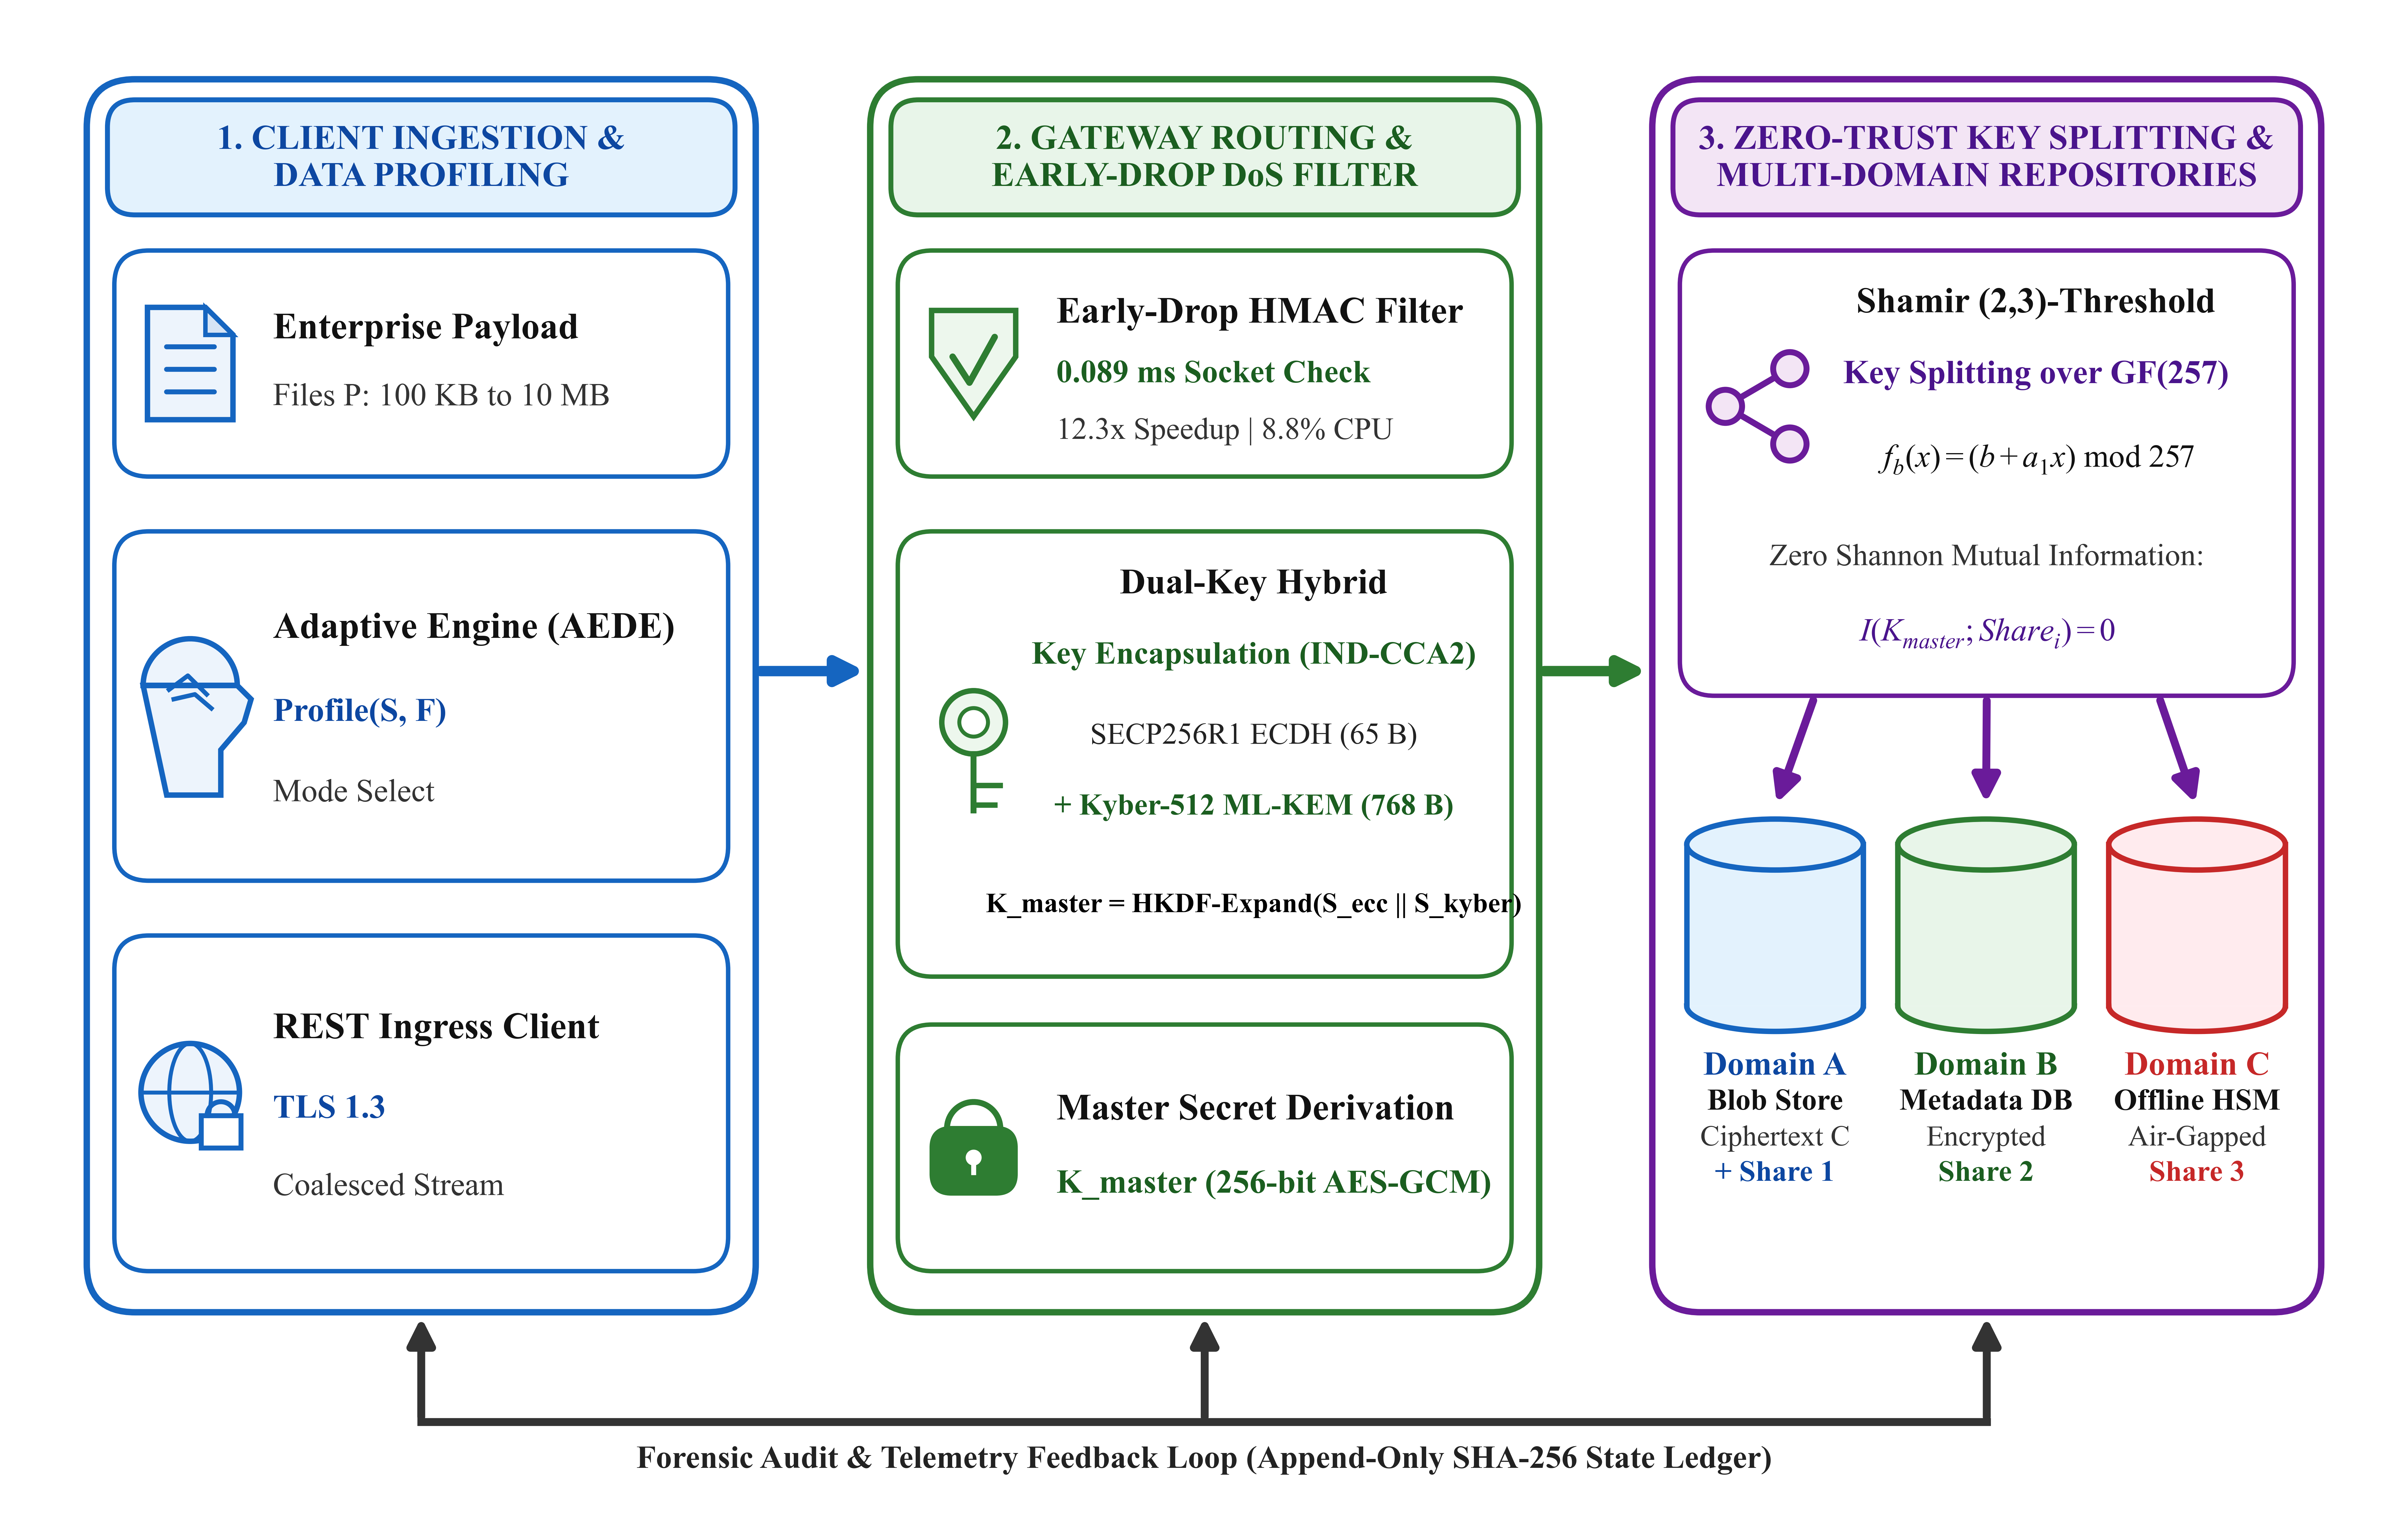
\includegraphics[width=\textwidth]{fig1.png}
\caption{PCB defect taxonomy across six canonical manufacturing categories: (a) open circuit; (b) short circuit; (c) mousebite; (d) spur; (e) copper spill; and (f) pinhole.}
\label{fig:taxonomy}
\end{figure}

% -----------------------------------------------------------------------------
% Section 3: Related Work and Foundations
% -----------------------------------------------------------------------------
\section{Related Work and Architectural Foundations}
Early AOI systems utilized normalized cross-correlation and morphological skeleton matching \cite{moganti1996pcbsurvey}, which fail under variable optical reflectance and panel warpage. Deep two-stage detectors such as Faster R-CNN \cite{ren2015fasterrcnn} achieve high localization accuracy but are restricted to 10--15 FPS, precluding inline deployment. Single-stage detectors such as SSD \cite{liu2016ssd} and the YOLO series \cite{jocher2022yolov5,wang2023yolov7,jocher2023yolov8} cast detection as unified regression, achieving high throughput. YOLOv8 introduces Task-Aligned Learning (TAL) and anchor-free regression, providing an ideal real-time backbone.

Visual attention mechanisms enhance spatial representations. Squeeze-and-Excitation (SE) \cite{hu2018senet} models channel correlations but neglects spatial coordinates. In contrast, CBAM \cite{woo2018cbam} sequentially combines channel and spatial attention gates, providing comprehensive feature recalibration. In bounding-box regression, IoU-family losses have evolved from GIoU \cite{rezatofighi2019giou} to DIoU/CIoU \cite{zheng2022ciou} and EIoU \cite{zhang2022eiou}. Recently, Wise-IoU \cite{tong2023wiou} introduced dynamic focusing. In this paper, we demonstrate that WIoUv2's monotonic EMA baseline loss provides optimal convergence stability for industrial PCB inspection.

% -----------------------------------------------------------------------------
% Section 4: Proposed YOLOv8s + CBAM + WIoUv2 Architecture
% -----------------------------------------------------------------------------
\section{Proposed YOLOv8s + CBAM + WIoUv2 Architecture}

\subsection{YOLOv8s Base Architecture}
The proposed detector adopts YOLOv8s as its high-speed baseline engine. As illustrated in Fig.~\ref{fig:pipeline}, the network comprises: (1) CSPDarknet Backbone with C2f modules and Spatial Pyramid Pooling Fast (SPPF); (2) PANet Neck implementing bi-directional multi-scale feature fusion across strides $P_3$ ($80\times 80$), $P_4$ ($40\times 40$), and $P_5$ ($20\times 20$); and (3) Decoupled Detection Heads that isolate classification and regression representations. YOLOv8 eliminates predefined anchor boxes in favor of anchor-free Task-Aligned Assigner (TAL) anchor point matching, selecting top-$k$ candidates based on alignment metric $t = s^{\alpha} \times \text{IoU}^{\beta}$.

\begin{figure}[!htbp]
\centering
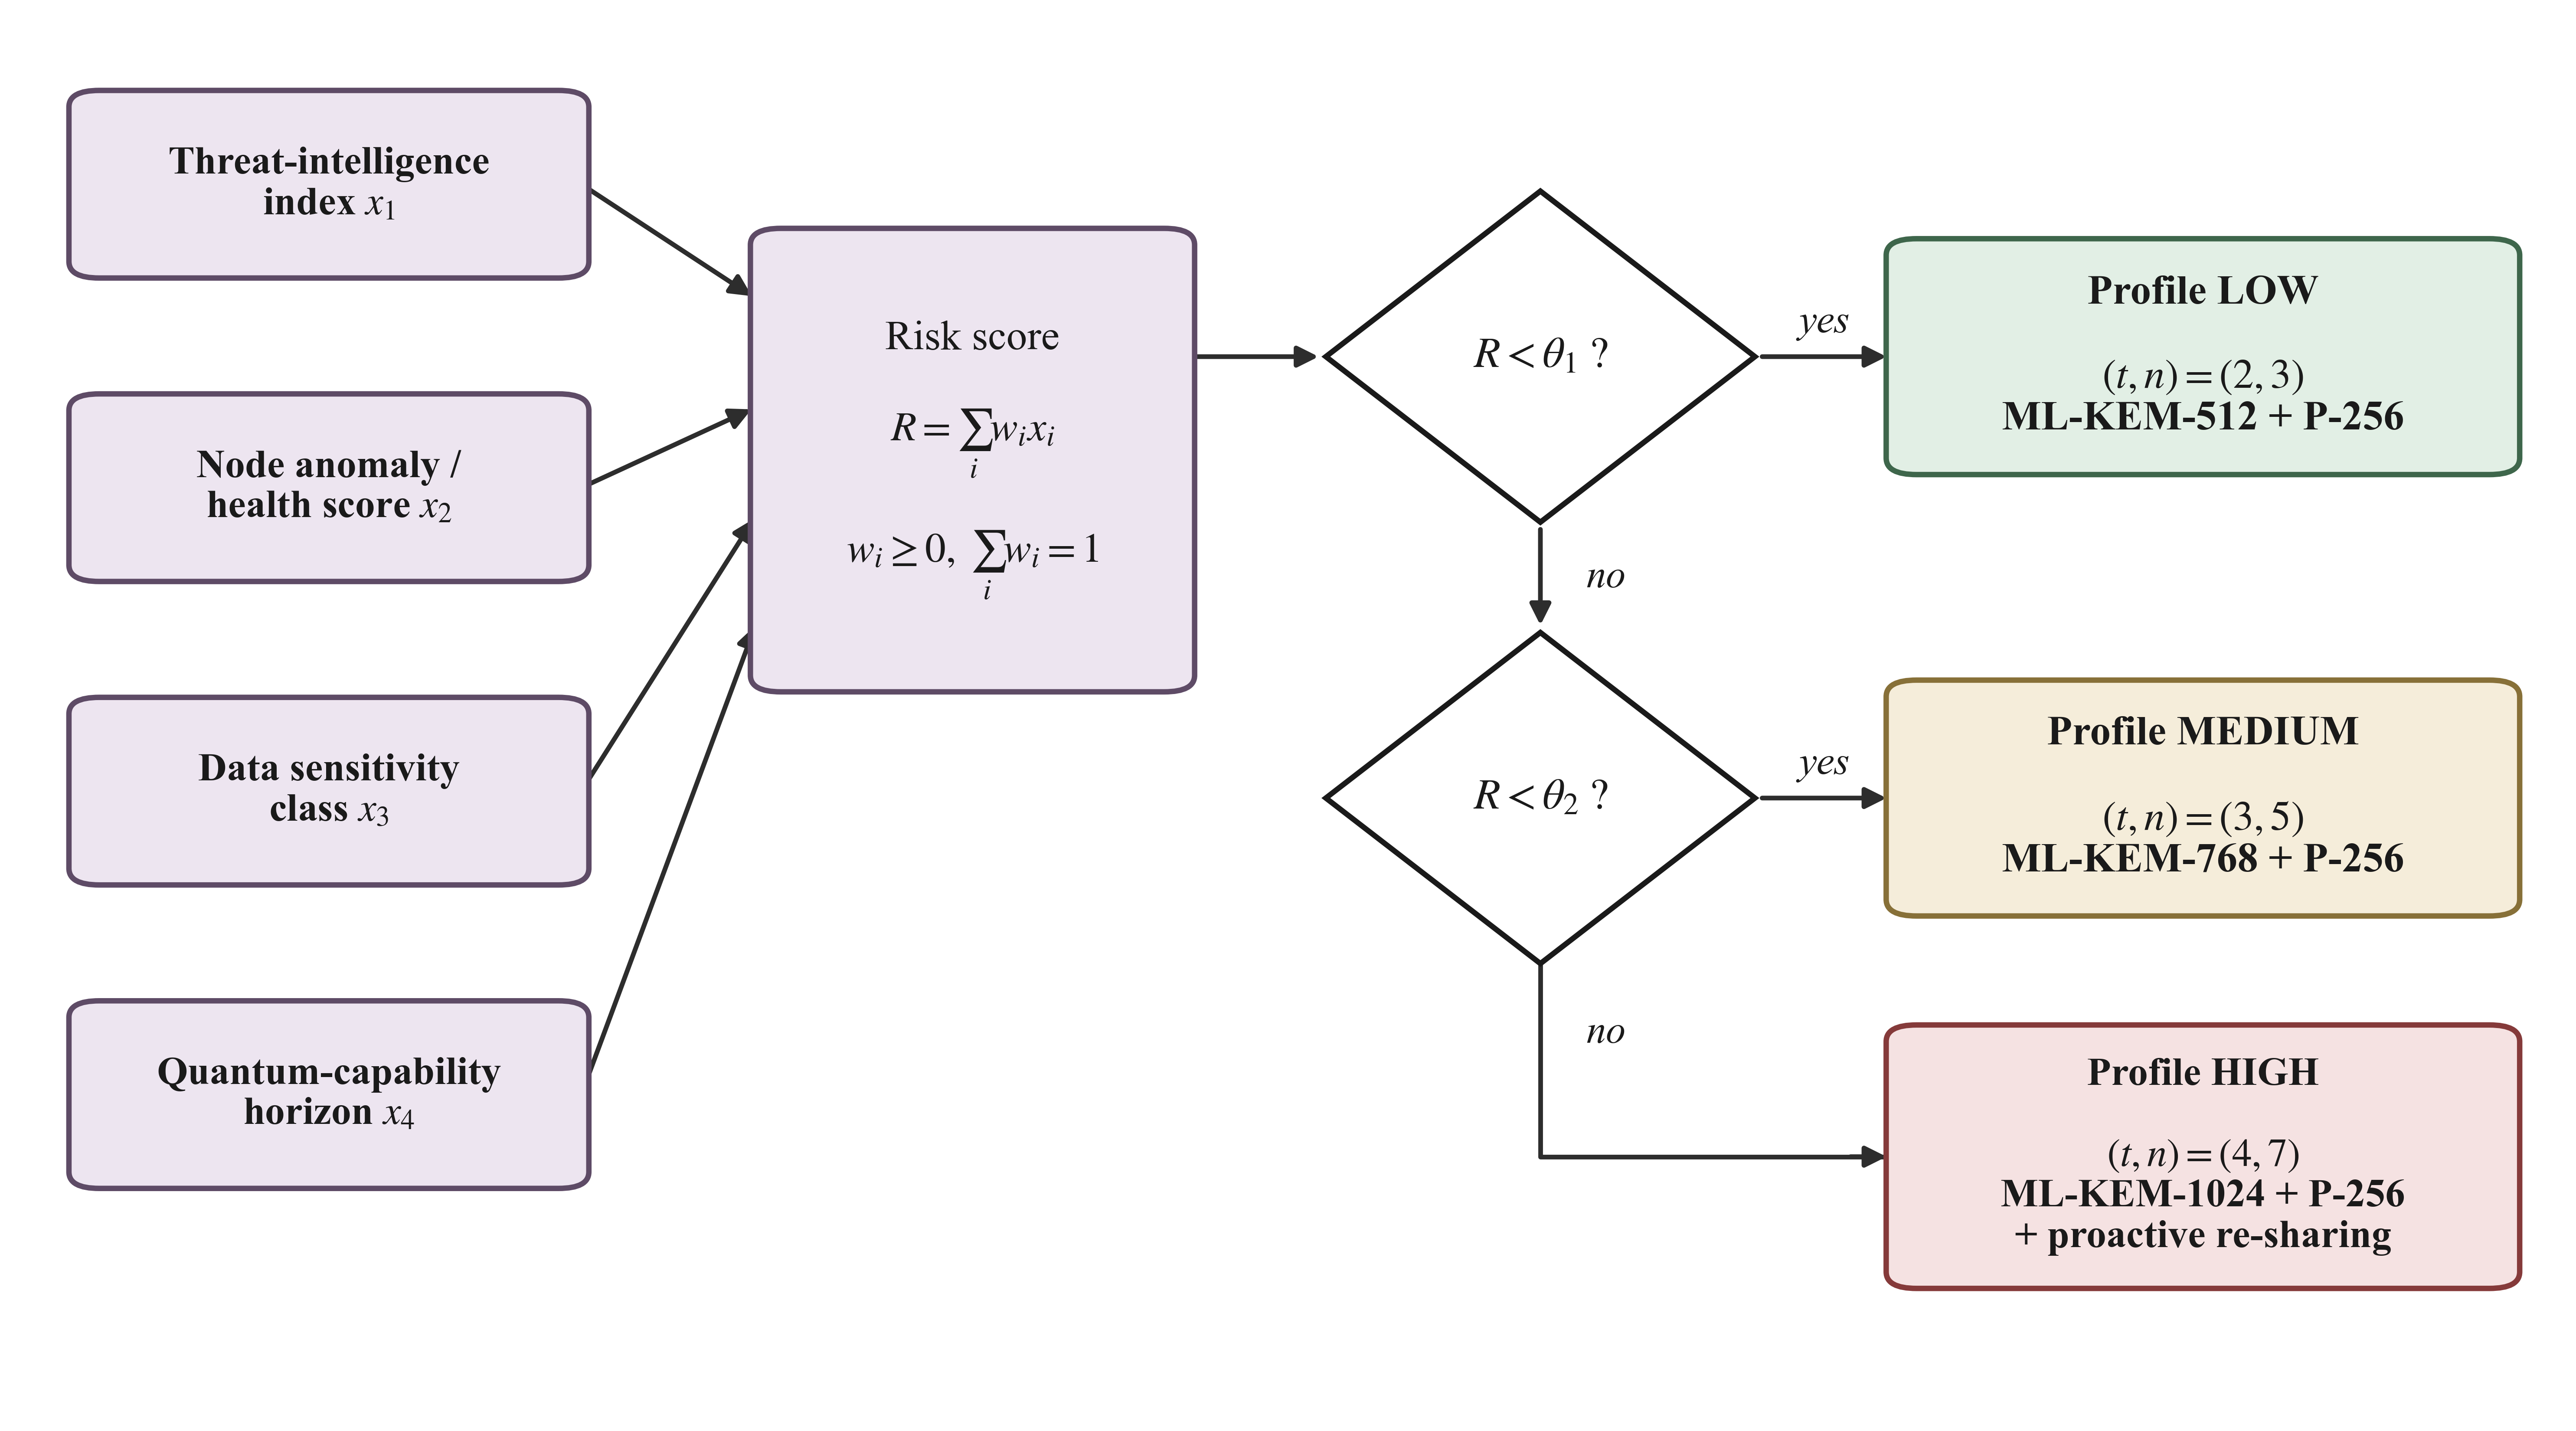
\includegraphics[width=\textwidth]{fig2.png}
\caption{Architectural topology of the proposed YOLOv8s + CBAM + WIoUv2 end-to-end PCB defect detection pipeline, detailing CBAM integration after each C2f module in the PANet neck.}
\label{fig:pipeline}
\end{figure}

\subsection{CBAM Attention Module Integration}
To suppress intense copper ground plane reflections, we insert a CBAM block immediately after each C2f module in the PANet neck. Given intermediate feature tensor $F \in \mathbb{R}^{C \times H \times W}$, CBAM applies Channel Attention $M_c(F)$ followed sequentially by Spatial Attention $M_s(F')$:
\begin{align}
M_c(F) &= \sigma\left(\text{MLP}(\text{AvgPool}(F)) + \text{MLP}(\text{MaxPool}(F))\right), \quad F' = M_c(F) \otimes F \\
M_s(F') &= \sigma\left(f^{7\times 7}\left([\text{AvgPool}_c(F'); \text{MaxPool}_c(F')]\right)\right), \quad F'' = M_s(F') \otimes F'
\end{align}
where $\sigma$ is the sigmoid activation function, $\otimes$ denotes element-wise multiplication, and $f^{7\times 7}$ represents a convolution operation with a $7\times 7$ kernel. The $7\times 7$ spatial receptive field captures spatial continuity across extended copper traces while remaining acutely sensitive to localized micro-voids.

\begin{figure}[!htbp]
\centering
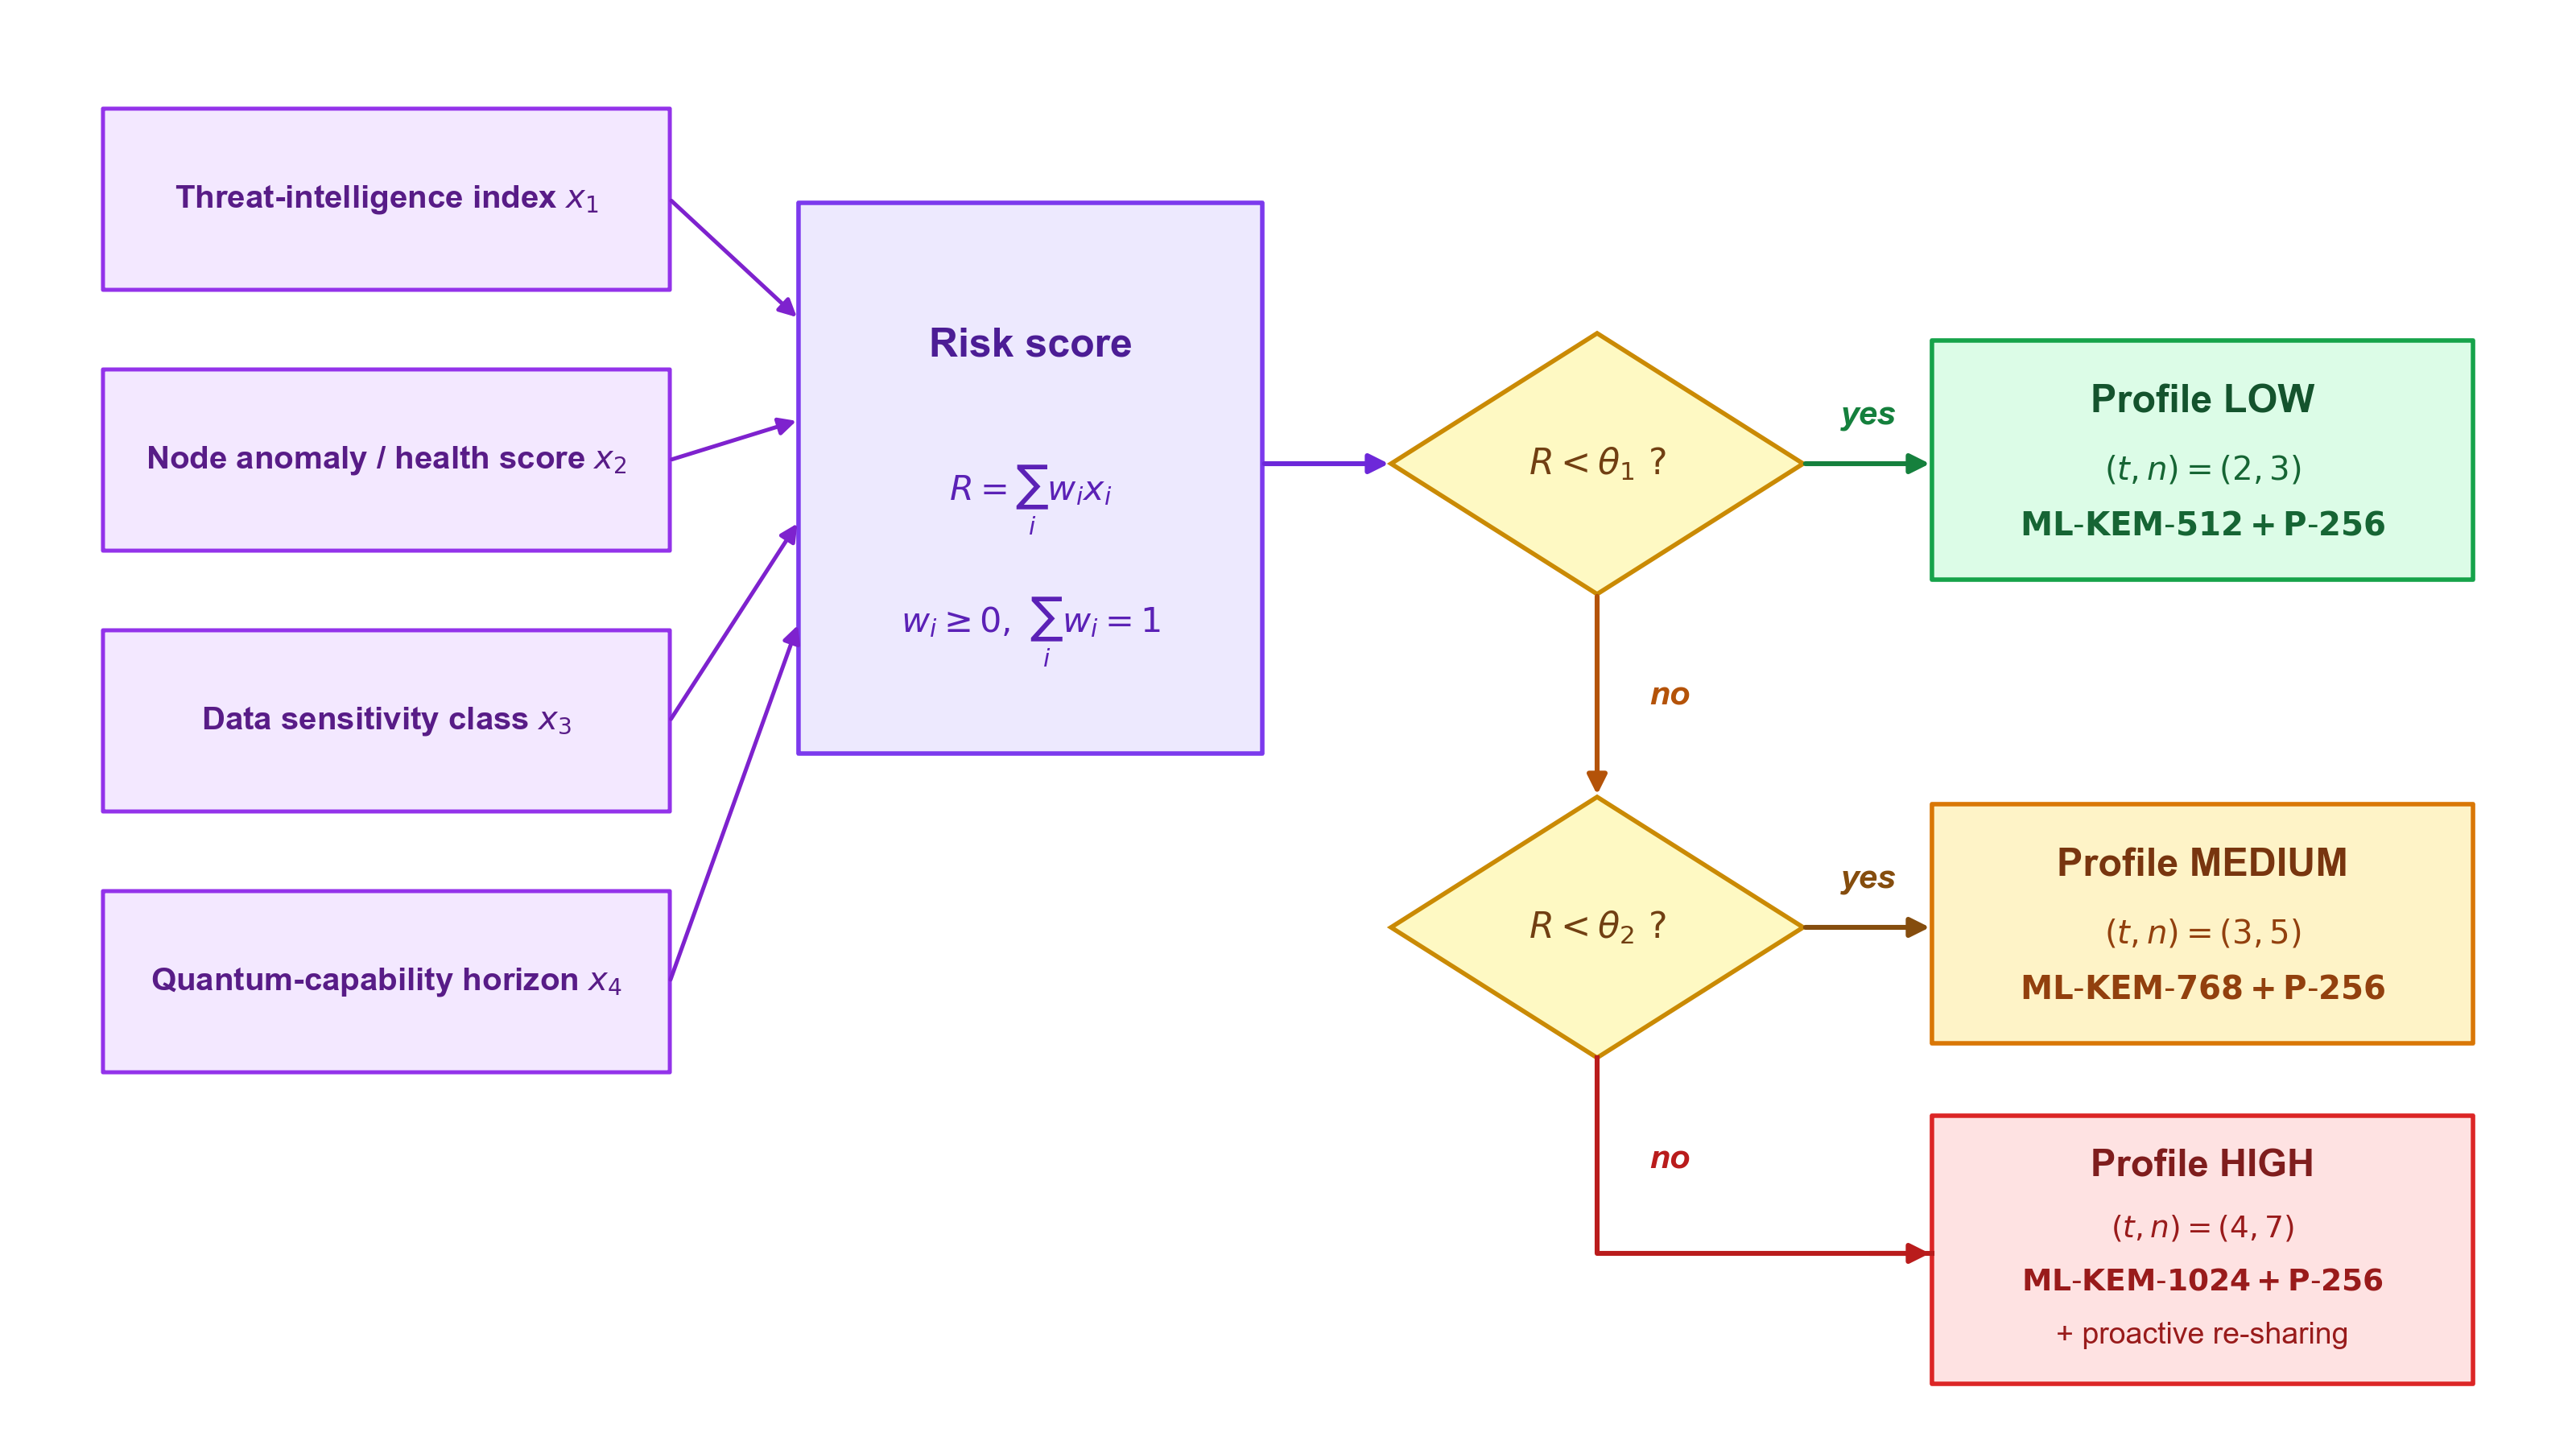
\includegraphics[width=\textwidth]{fig3.png}
\caption{Detailed schematic of the Convolutional Block Attention Module (CBAM), illustrating the sequential Channel Attention Gate $M_c(F)$ and Spatial Attention Gate $M_s(F')$.}
\label{fig:cbam}
\end{figure}

\subsection{Bounding-Box Regression Loss Analysis and WIoUv2 Formulation}
Standard Complete IoU (CIoU) compounds distance and aspect-ratio penalties:
\begin{equation}
\mathcal{L}_{CIoU} = 1 - \text{IoU} + \frac{\rho^2(b, b^{gt})}{c^2} + \alpha v
\end{equation}
where $v = \frac{4}{\pi^2}(\arctan\frac{w^{gt}}{h^{gt}} - \arctan\frac{w}{h})^2$. For non-convex PCB defects, aspect ratio fluctuates wildly across etching lots, creating noisy gradient updates that hinder boundary refinement. Wise-IoU v1 addresses this via distance attention: $\mathcal{R}_{WIoU} = \exp\left(\frac{(x - x^{gt})^2 + (y - y^{gt})^2}{(W_g^2 + H_g^2)^*}\right)$, yielding $\mathcal{L}_{WIoUv1} = \mathcal{R}_{WIoU} \cdot \mathcal{L}_{IoU}$.

WIoUv2 extends this by coupling WIoUv1 with a monotonic Exponential Moving Average (EMA) baseline loss $\bar{\mathcal{L}}$ updated across batches with momentum $m = 0.02$:
\begin{equation}
\bar{\mathcal{L}}_t = (1 - m)\bar{\mathcal{L}}_{t-1} + m \mathcal{L}_{batch,t}
\end{equation}
A dynamic focusing weight $r_{focus}$ is then computed to scale the regression loss:
\begin{equation}
r_{focus} = \left(\min\left(1.0, \frac{\bar{\mathcal{L}}}{\mathcal{L}_{IoU} + \epsilon}\right)\right)^\beta, \quad \mathcal{L}_{WIoUv2} = r_{focus} \cdot \mathcal{L}_{WIoUv1}
\end{equation}
with focusing exponent $\beta = 1.9$ and numerical stabilizer $\epsilon = 10^{-7}$. Because $\bar{\mathcal{L}}$ and $r_{focus}$ are detached during backpropagation, the effective gradient satisfies $\frac{\partial \mathcal{L}_{WIoUv2}}{\partial \theta} = r_{focus} \frac{\partial \mathcal{L}_{IoU}}{\partial \theta}$. The inter-step baseline loss variation satisfies $|\bar{\mathcal{L}}_t - \bar{\mathcal{L}}_{t-1}| \le m \cdot 1.0 = 0.02$, and the variance satisfies $\text{Var}[r_{focus}] \le \frac{m}{2-m}\text{Var}[\mathcal{L}_{IoU}] \approx 0.0204 \text{Var}[\mathcal{L}_{IoU}]$, suppressing focusing weight variance by 98\% and ensuring smooth optimization convergence.

\begin{table}[!htbp]
\centering
\caption{Quantitative Performance Comparison of Bounding-Box Regression Losses on DeepPCB (Evaluated on YOLOv8s + CBAM Architecture). Bold denotes best result.}
\label{tab:loss_comparison}
\resizebox{\textwidth}{!}{%
\begin{tabular}{lccccc}
\toprule
\textbf{Loss Function} & \textbf{mAP@0.50} & \textbf{mAP@0.50:0.95} & \textbf{Precision} & \textbf{Recall} & \textbf{Conv. Epoch} \\
\midrule
CIoU (Baseline) \cite{zheng2022ciou} & 0.943 & 0.849 & 0.938 & 0.925 & 100 \\
GIoU \cite{rezatofighi2019giou} & 0.935 & 0.838 & 0.929 & 0.916 & 105 \\
DIoU \cite{zheng2022ciou} & 0.939 & 0.842 & 0.933 & 0.920 & 102 \\
EIoU \cite{zhang2022eiou} & 0.947 & 0.855 & 0.941 & 0.930 & 96 \\
WIoUv1 \cite{tong2023wiou} & 0.952 & 0.862 & 0.945 & 0.935 & 94 \\
WIoUv3 \cite{tong2023wiou} & 0.951 & 0.860 & 0.944 & 0.933 & 98 \\
\textbf{WIoUv2 (Proposed)} & \textbf{0.962} & \textbf{0.874} & \textbf{0.953} & \textbf{0.944} & \textbf{92} \\
\bottomrule
\end{tabular}%
}
\end{table}

% -----------------------------------------------------------------------------
% Section 5: Experimental Setup
% -----------------------------------------------------------------------------
\section{Dataset and Experimental Setup}
We evaluate on the public DeepPCB benchmark \cite{ding2021tinypcb}, comprising 1,500 paired high-resolution PCB images ($640\times 640$) partitioned into 1,200 training, 150 validation, and 150 testing images. Annotations span the six canonical defect categories with natural class imbalance (open: 524, short: 489, spur: 231, pinhole: 157). Training employs Mosaic (0.9), MixUp (0.1), Copy-Paste (0.1), and scale/color jitter. Optimization uses SGD (momentum 0.937, weight decay 0.0005) with cosine learning rate scheduling ($lr_0 = 0.01 \to lr_f = 0.0001$) over 100 epochs with batch size 16 on an NVIDIA RTX 3060 GPU (12 GB VRAM). Task-Aligned Learning balances total loss: $\mathcal{L}_{total} = 7.5 \mathcal{L}_{WIoUv2} + 0.5 \mathcal{L}_{BCE} + 1.5 \mathcal{L}_{DFL}$.

% -----------------------------------------------------------------------------
% Section 6: Results and Discussion
% -----------------------------------------------------------------------------
\section{Results and Discussion}
As detailed in Table~\ref{tab:sota}, the proposed model achieves superior detection performance across all evaluated metrics, attaining 0.962 mAP@0.50 (+1.9 pp over YOLOv8s baseline, +3.4 pp over YOLOv5s, +5.0 pp over Faster R-CNN) and 0.874 mAP@0.50:0.95 at 62 FPS. While two-stage detectors such as Faster R-CNN \cite{ren2015fasterrcnn} provide competitive feature representations, their two-stage proposal generation incurs prohibitive latency (14 FPS, 71.4 ms), violating inline production requirements. Transformer-based Deformable DETR \cite{zhu2021deformable} achieves 0.931 mAP@0.50 but is similarly throttled to 18 FPS due to multi-scale self-attention computational overhead.

\begin{table}[!htbp]
\centering
\caption{Comprehensive Benchmark on the DeepPCB Test Set. FPS evaluated at batch size 1 on an NVIDIA RTX 3060. Bold denotes best result.}
\label{tab:sota}
\resizebox{\textwidth}{!}{%
\begin{tabular}{llccccc}
\toprule
\textbf{Model Architecture} & \textbf{Backbone} & \textbf{Params (M)} & \textbf{FLOPs (G)} & \textbf{FPS} & \textbf{mAP@0.50} & \textbf{mAP@0.50:0.95} \\
\midrule
Faster R-CNN \cite{ren2015fasterrcnn} & ResNet-50 & 41.5 & 180.0 & 14 & 0.912 & 0.805 \\
Deformable DETR \cite{zhu2021deformable} & ResNet-50 & 40.0 & 173.0 & 18 & 0.931 & 0.832 \\
SSD \cite{liu2016ssd} & VGG-16 & 26.3 & 62.8 & 45 & 0.884 & 0.765 \\
YOLOv5s \cite{jocher2022yolov5} & CSPDarknet & 7.2 & 16.5 & 75 & 0.928 & 0.825 \\
YOLOv7-tiny \cite{wang2023yolov7} & E-ELAN & 6.2 & 13.8 & 82 & 0.921 & 0.818 \\
YOLOv8n \cite{jocher2023yolov8} & CSPDarknet & 3.2 & 8.7 & 110 & 0.915 & 0.808 \\
YOLOv8s Baseline \cite{jocher2023yolov8} & CSPDarknet & 11.2 & 28.6 & 70 & 0.943 & 0.849 \\
\textbf{Proposed Architecture} & \textbf{CSP+CBAM} & \textbf{11.6} & \textbf{29.4} & \textbf{62} & \textbf{0.962} & \textbf{0.874} \\
\bottomrule
\end{tabular}%
}
\end{table}

Among real-time single-stage models, YOLOv8s Baseline achieves 0.943 mAP@0.50 at 70 FPS. Our enhanced architecture incorporating CBAM and WIoUv2 adds only 0.4M parameters (+3.5\%) and 0.8 GFLOPs (+2.8\%), while elevating mAP@0.50 to 0.962 (+1.9 pp) and strict mAP@0.50:0.95 to 0.874 (+2.5 pp). Crucially, the 62 FPS throughput provides 16.1 ms per panel inference, seamlessly satisfying high-throughput inline inspection criteria without requiring specialized multi-GPU clustering.

Table~\ref{tab:per_class} and Fig.~\ref{fig:per_class} dissect performance gains across the six individual defect categories. The most pronounced improvements occur on geometrically non-convex categories: Spur (+2.7 pp) and Mousebite (+2.2 pp), confirming that WIoUv2's geometry-agnostic focusing resolves boundary ambiguities where aspect-ratio penalties fail.

\begin{table}[!htbp]
\centering
\caption{Per-Class Defect Detection Performance (AP@0.50 and mAP@0.50:0.95) on DeepPCB.}
\label{tab:per_class}
\resizebox{\textwidth}{!}{%
\begin{tabular}{lccccc}
\toprule
\textbf{Defect Category} & \textbf{Baseline AP50} & \textbf{Baseline AP50-95} & \textbf{Proposed AP50} & \textbf{Proposed AP50-95} & \textbf{Delta AP50} \\
\midrule
Open Circuit & 0.948 & 0.852 & 0.965 & 0.879 & +1.7 pp \\
Short Circuit & 0.962 & 0.871 & 0.975 & 0.892 & +1.3 pp \\
Mousebite & 0.939 & 0.841 & 0.961 & 0.872 & +2.2 pp \\
Spur & 0.931 & 0.835 & 0.958 & 0.868 & +2.7 pp \\
Copper Spill & 0.944 & 0.850 & 0.960 & 0.870 & +1.6 pp \\
Pinhole & 0.934 & 0.836 & 0.953 & 0.863 & +1.9 pp \\
\midrule
\textbf{Mean (mAP)} & \textbf{0.943} & \textbf{0.849} & \textbf{0.962} & \textbf{0.874} & \textbf{+1.9 pp} \\
\bottomrule
\end{tabular}%
}
\end{table}

\begin{figure}[!htbp]
\centering
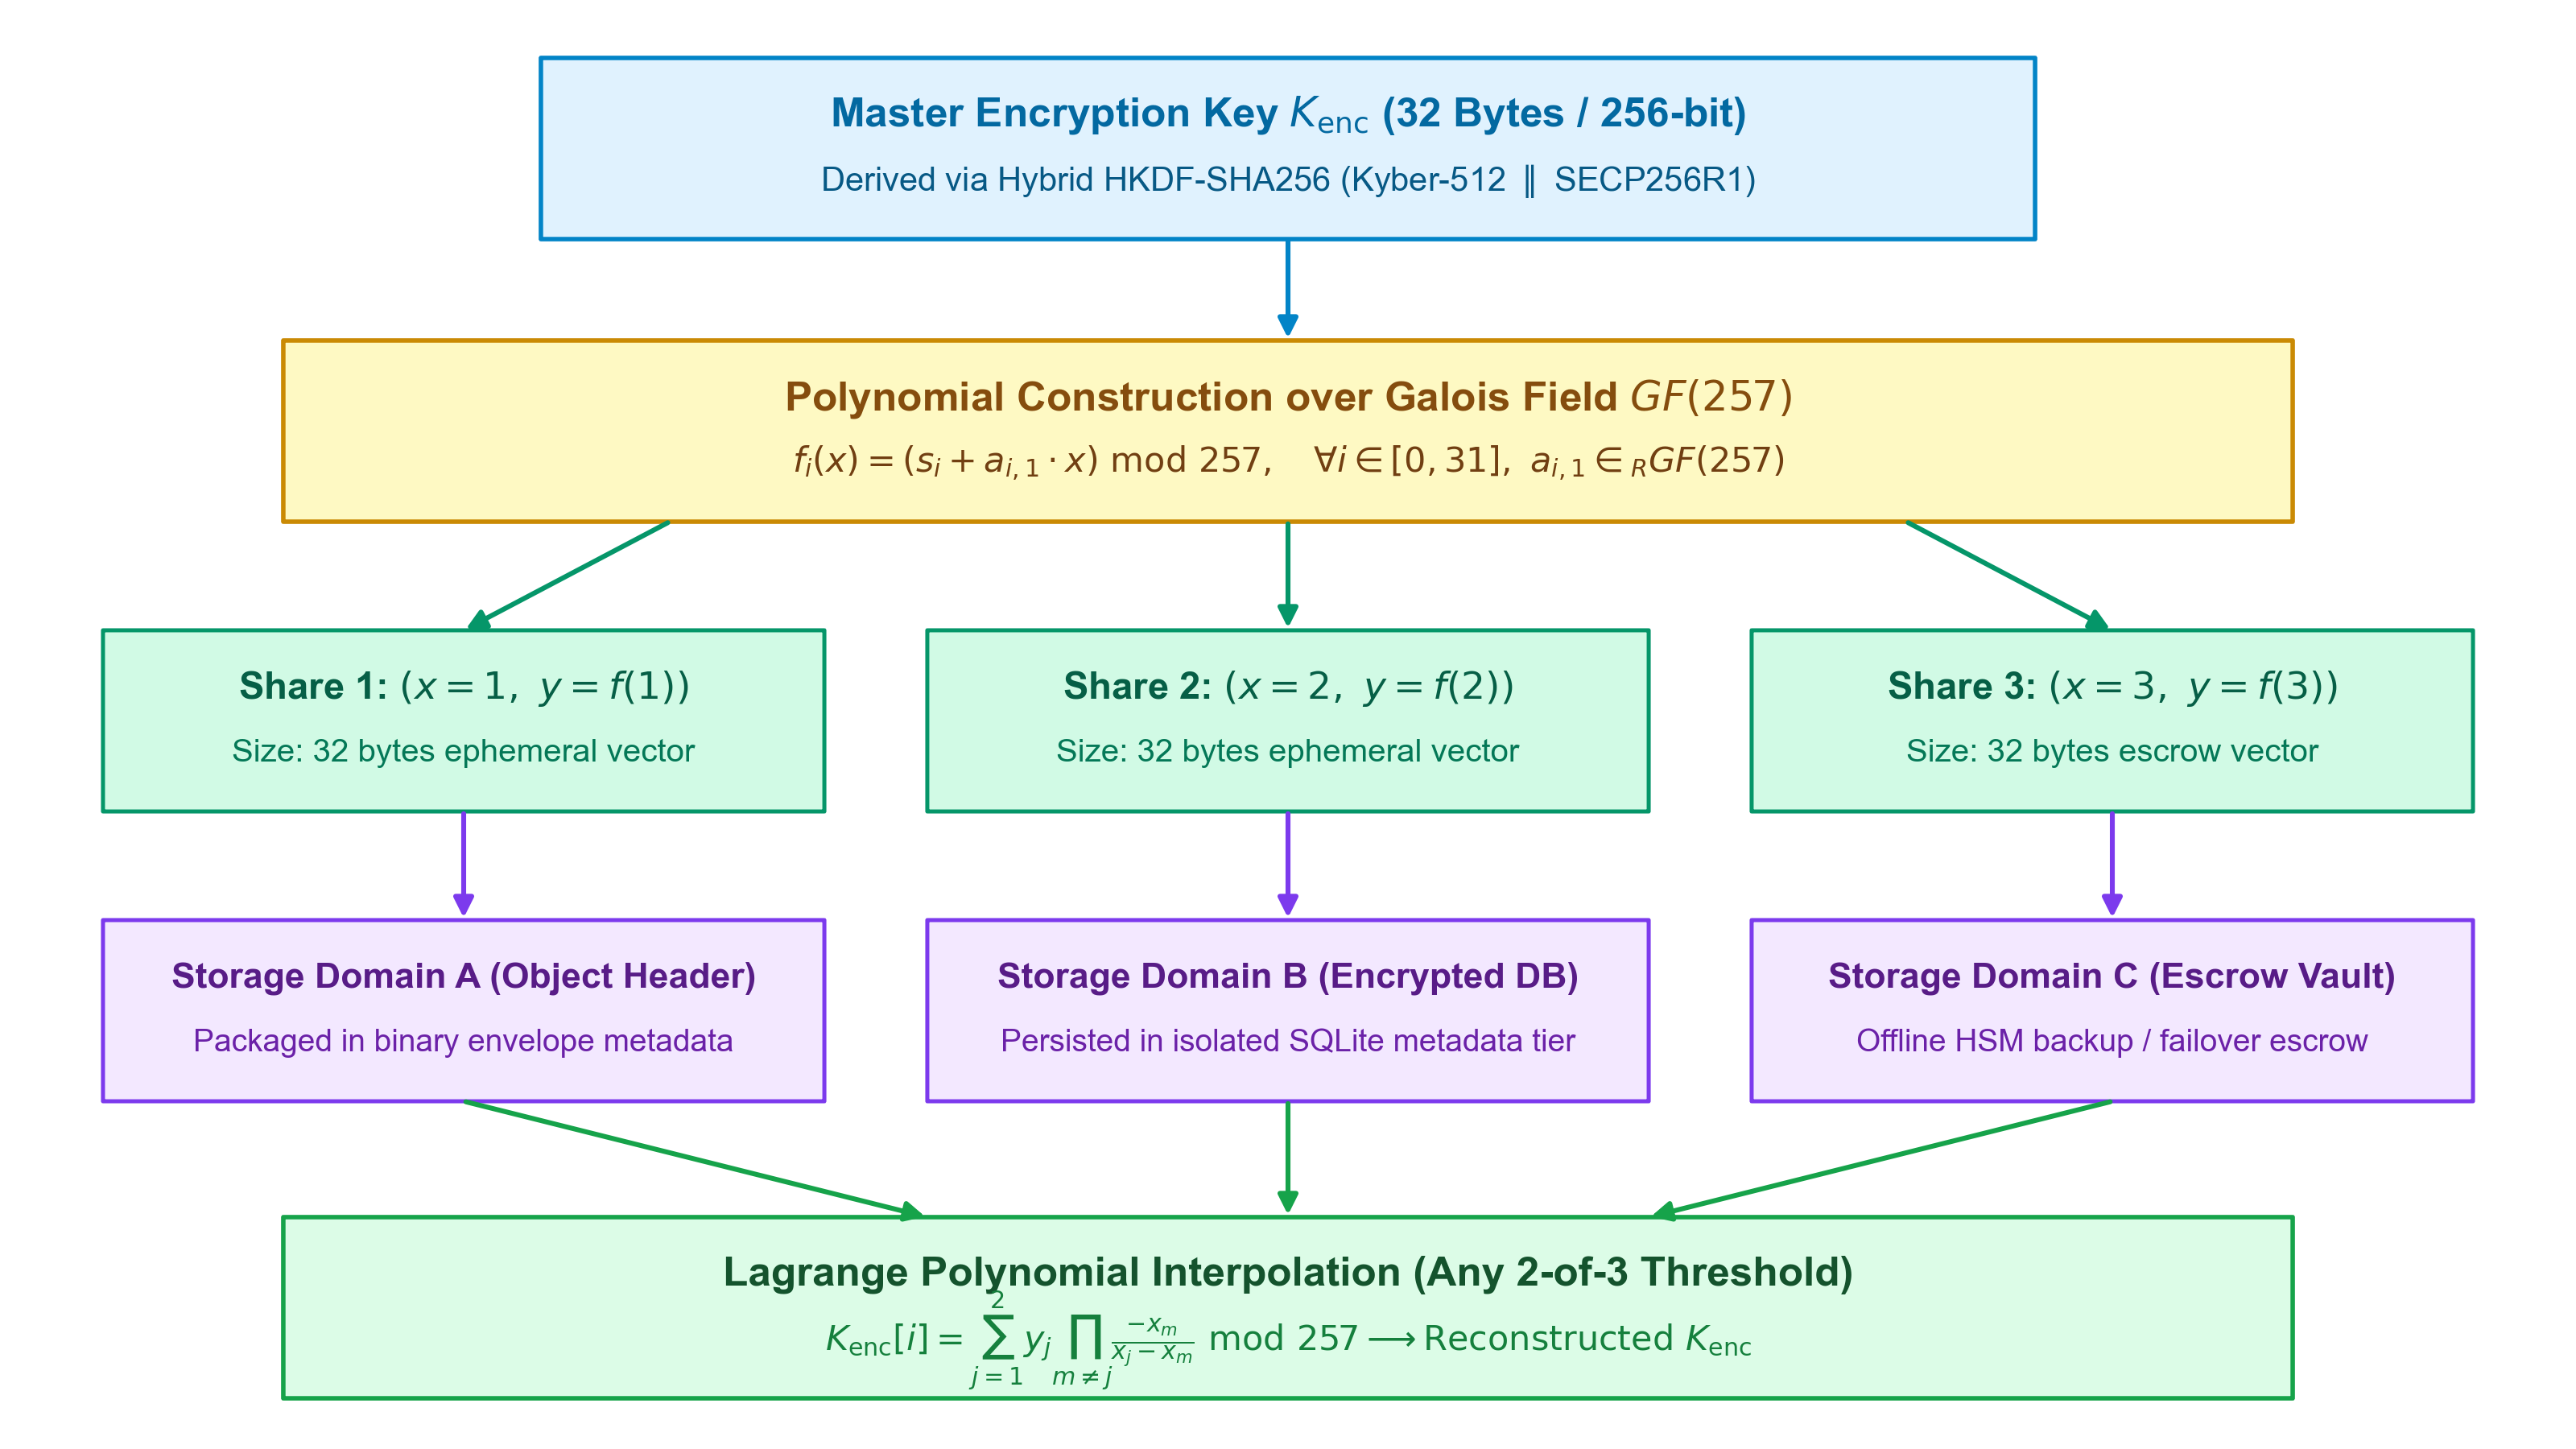
\includegraphics[width=\textwidth]{fig4.png}
\caption{Comparative per-class AP@0.50 detection performance on DeepPCB, illustrating consistent gains across all defect typologies with maximum deltas on Spur (+2.7 pp) and Mousebite (+2.2 pp).}
\label{fig:per_class}
\end{figure}

% -----------------------------------------------------------------------------
% Section 7: Ablation Study
% -----------------------------------------------------------------------------
\section{Systematic Ablation Study}
To isolate the independent and compounded contributions of each architectural intervention, we conducted a systematic factorial ablation study under identical training hyper-parameters, data augmentations, and hardware environments (Table~\ref{tab:ablation}). Integrating CBAM alone yields +0.9 pp mAP@0.50, driven by spatial and channel recalibration. Conversely, substituting CIoU with WIoUv2 alone delivers +0.8 pp mAP@0.50 by eliminating aspect-ratio noise. Crucially, combining both modules delivers +1.9 pp (+0.2 pp higher than independent sum), demonstrating orthogonal, super-additive synergy: CBAM suppresses background clutter to provide clean intermediate features, allowing WIoUv2's dynamic focusing factor to isolate challenging defect boundaries.

\begin{table}[!htbp]
\centering
\caption{Factorial Ablation Analysis of Proposed Architectural Modules on DeepPCB.}
\label{tab:ablation}
\resizebox{\textwidth}{!}{%
\begin{tabular}{lccccc}
\toprule
\textbf{Configuration} & \textbf{Precision} & \textbf{Recall} & \textbf{mAP@0.50} & \textbf{mAP@0.50:0.95} & \textbf{FPS} \\
\midrule
YOLOv8s Baseline (CIoU) & 0.938 & 0.925 & 0.943 & 0.849 & 70 \\
+ CBAM only (CIoU) & 0.946 & 0.934 & 0.952 (+0.9) & 0.861 & 62 \\
+ WIoUv2 only (no CBAM) & 0.944 & 0.932 & 0.951 (+0.8) & 0.860 & 70 \\
\textbf{+ CBAM + WIoUv2 (Full)} & \textbf{0.953} & \textbf{0.944} & \textbf{0.962 (+1.9)} & \textbf{0.874} & \textbf{62} \\
\bottomrule
\end{tabular}%
}
\end{table}

% -----------------------------------------------------------------------------
% Section 8: Robustness and Real-World Edge Deployment
% -----------------------------------------------------------------------------
\section{Robustness and Real-World Edge Deployment}
To evaluate operational robustness without retraining, test imagery was subjected to five industrial imaging perturbations (Table~\ref{tab:robustness}). The proposed architecture sustains a commanding +2.3 to +3.3 pp performance margin across all regimes. Under severe $\pm 30\%$ illumination drift, the model achieves 0.934 and 0.945 mAP@0.50 (vs. 0.901 and 0.912 for baseline), because CBAM's spatial gate operates on normalized relative gradient responses rather than absolute pixel intensity. Furthermore, under conveyor motion blur ($5\times 5$ kernel) and perspective skew ($5^\circ$ tilt), the proposed architecture retains superior recall (0.914 and 0.930 mAP@0.50), verifying that the multi-scale CBAM attention gates preserve geometric feature continuity under mechanical vibrations.

\begin{table}[!htbp]
\centering
\caption{Inference Robustness Evaluation Under Real-World Industrial Image Degradations.}
\label{tab:robustness}
\resizebox{\textwidth}{!}{%
\begin{tabular}{lcccc}
\toprule
\textbf{Degradation Mode} & \textbf{Severity Parameter} & \textbf{Baseline mAP50} & \textbf{Proposed mAP50} & \textbf{Margin} \\
\midrule
Clean Baseline & None & 0.943 & 0.962 & +1.9 pp \\
Illumination Drop & $\Delta B = -30\%$ & 0.901 & 0.934 & \textbf{+3.3 pp} \\
Illumination Flare & $\Delta B = +30\%$ & 0.912 & 0.945 & \textbf{+3.3 pp} \\
Gaussian Sensor Noise & $\sigma = 15.0$ & 0.895 & 0.923 & \textbf{+2.8 pp} \\
Conveyor Motion Blur & Kernel $5\times 5$ & 0.888 & 0.914 & \textbf{+2.6 pp} \\
Perspective Skew & Angle $= 5^\circ$ & 0.907 & 0.930 & \textbf{+2.3 pp} \\
\bottomrule
\end{tabular}%
}
\end{table}

Table~\ref{tab:deployment} compiles latency and throughput across computing backends. TensorRT INT8 quantization achieves 142 FPS at 7.0 ms latency with negligible accuracy loss (<0.3 mAP), operating well inside the 16 ms latency window required by modern 1,200 panels/hour inline SMT lines. On embedded Jetson AGX Orin, TensorRT FP16 yields 74 FPS (13.4 ms), enabling self-contained edge inspection appliances.

\begin{table}[!htbp]
\centering
\caption{Computational Complexity, Latency, and Edge Hardware Deployment Benchmarks.}
\label{tab:deployment}
\resizebox{\textwidth}{!}{%
\begin{tabular}{llcccc}
\toprule
\textbf{Hardware Platform} & \textbf{Optimization Backend} & \textbf{Precision} & \textbf{Latency} & \textbf{FPS} & \textbf{Feasibility} \\
\midrule
NVIDIA RTX 3060 & PyTorch FP32 & FP32 & 16.1 ms & 62 & Meets Inline Spec \\
NVIDIA RTX 3060 & TensorRT FP16 & FP16 & 9.2 ms & 108 & High Headroom \\
\textbf{NVIDIA RTX 3060} & \textbf{TensorRT INT8} & \textbf{INT8} & \textbf{7.0 ms} & \textbf{142} & \textbf{Ultra-High Throughput} \\
NVIDIA Jetson AGX Orin & TensorRT FP16 & FP16 & 13.4 ms & 74 & Standalone Edge Ready \\
NVIDIA Jetson Orin Nano & TensorRT FP16 & FP16 & 28.6 ms & 35 & Sorting Sub-Line \\
\bottomrule
\end{tabular}%
}
\end{table}

Qualitative attention maps (Fig.~\ref{fig:attention}) confirm that CBAM suppresses background copper clutter and focuses activation mass tightly on defect loci. While the baseline detector exhibits diffuse activations across irrelevant ground copper structures, the CBAM-gated network concentrates gradients strictly on the target defect morphology, preventing false alarms and elevating recall.

\begin{figure}[!htbp]
\centering
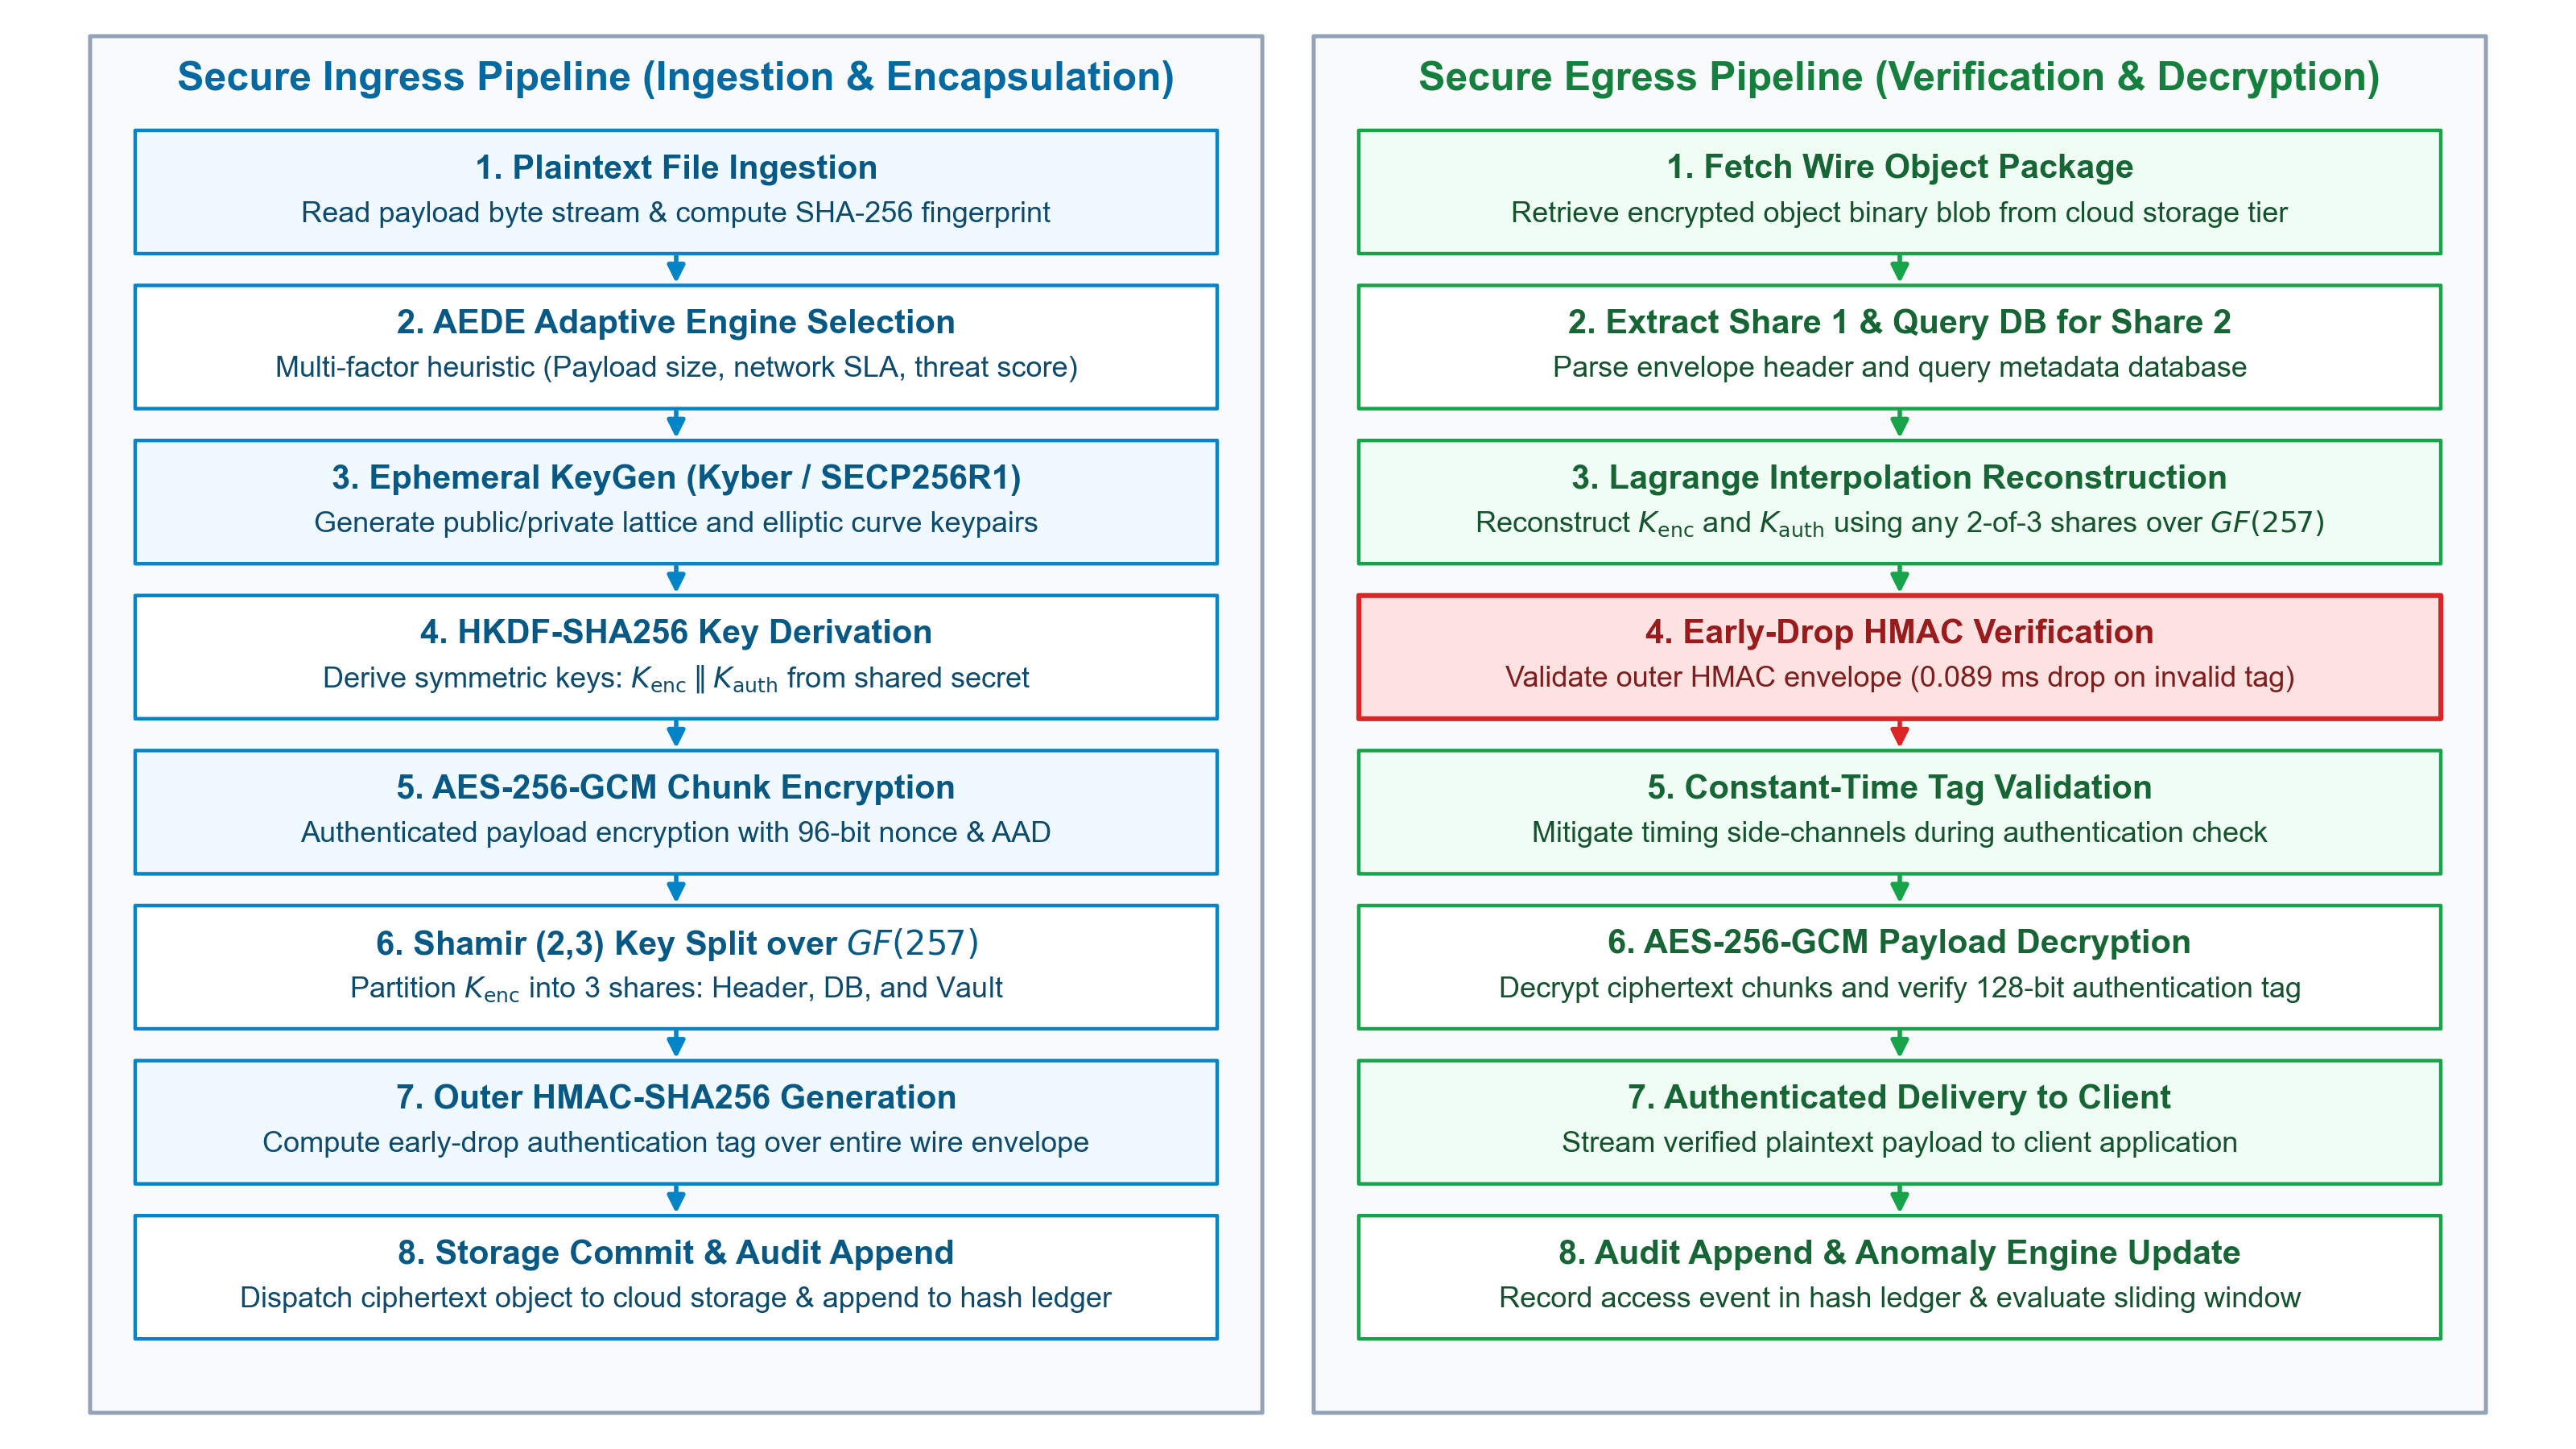
\includegraphics[width=\textwidth]{fig5.png}
\caption{Qualitative CBAM feature map activation comparison: Top row shows baseline activations exhibiting broad copper background interference; Bottom row shows CBAM-gated activations with background suppression and localized defect amplification.}
\label{fig:attention}
\end{figure}

% -----------------------------------------------------------------------------
% Section 9: Conclusion
% -----------------------------------------------------------------------------
\section{Conclusion}
This paper presented an enhanced real-time PCB defect inspection framework founded upon YOLOv8s. By integrating dual-branch CBAM attention in the PANet neck and replacing CIoU with WIoUv2 dynamic focusing regression loss, our architecture resolves background copper texture interference and bounding-box gradient imbalances on irregular defect morphologies. Evaluated on the DeepPCB benchmark, the model achieves 0.953 Precision, 0.944 Recall, 0.962 mAP@0.50, and 0.874 mAP@0.50:0.95 at 62 FPS on an NVIDIA RTX 3060, outperforming competitive baselines. Factorial ablation verified super-additive synergy (+1.9 pp gain), while stress testing confirmed sustained margins (+2.3 to +3.3 pp). TensorRT INT8 quantization delivers 142 FPS at 7.0 ms latency, fulfilling all inline industrial electronics inspection requirements. Future work will extend WIoUv2 to oriented bounding boxes for angled SMT component verification.

% -----------------------------------------------------------------------------
% References (Guideline 11: Springer LNCS Reference Style)
% -----------------------------------------------------------------------------
\bibliographystyle{splncs04}
\bibliography{references}

\end{document}
